\PassOptionsToPackage{unicode=true}{hyperref} % options for packages loaded elsewhere
\PassOptionsToPackage{hyphens}{url}
%
\documentclass[]{article}
\usepackage{lmodern}
\usepackage{amssymb,amsmath}
\usepackage{ifxetex,ifluatex}
\usepackage{fixltx2e} % provides \textsubscript
\ifnum 0\ifxetex 1\fi\ifluatex 1\fi=0 % if pdftex
  \usepackage[T1]{fontenc}
  \usepackage[utf8]{inputenc}
  \usepackage{textcomp} % provides euro and other symbols
\else % if luatex or xelatex
  \usepackage{unicode-math}
  \defaultfontfeatures{Ligatures=TeX,Scale=MatchLowercase}
\fi
% use upquote if available, for straight quotes in verbatim environments
\IfFileExists{upquote.sty}{\usepackage{upquote}}{}
% use microtype if available
\IfFileExists{microtype.sty}{%
\usepackage[]{microtype}
\UseMicrotypeSet[protrusion]{basicmath} % disable protrusion for tt fonts
}{}
\IfFileExists{parskip.sty}{%
\usepackage{parskip}
}{% else
\setlength{\parindent}{0pt}
\setlength{\parskip}{6pt plus 2pt minus 1pt}
}
\usepackage{hyperref}
\hypersetup{
            pdftitle={Kaggle Titanic Data Analysis Report},
            pdfauthor={P. Adames},
            pdfborder={0 0 0},
            breaklinks=true}
\urlstyle{same}  % don't use monospace font for urls
\usepackage[margin=1in]{geometry}
\usepackage{color}
\usepackage{fancyvrb}
\newcommand{\VerbBar}{|}
\newcommand{\VERB}{\Verb[commandchars=\\\{\}]}
\DefineVerbatimEnvironment{Highlighting}{Verbatim}{commandchars=\\\{\}}
% Add ',fontsize=\small' for more characters per line
\usepackage{framed}
\definecolor{shadecolor}{RGB}{248,248,248}
\newenvironment{Shaded}{\begin{snugshade}}{\end{snugshade}}
\newcommand{\AlertTok}[1]{\textcolor[rgb]{0.94,0.16,0.16}{#1}}
\newcommand{\AnnotationTok}[1]{\textcolor[rgb]{0.56,0.35,0.01}{\textbf{\textit{#1}}}}
\newcommand{\AttributeTok}[1]{\textcolor[rgb]{0.77,0.63,0.00}{#1}}
\newcommand{\BaseNTok}[1]{\textcolor[rgb]{0.00,0.00,0.81}{#1}}
\newcommand{\BuiltInTok}[1]{#1}
\newcommand{\CharTok}[1]{\textcolor[rgb]{0.31,0.60,0.02}{#1}}
\newcommand{\CommentTok}[1]{\textcolor[rgb]{0.56,0.35,0.01}{\textit{#1}}}
\newcommand{\CommentVarTok}[1]{\textcolor[rgb]{0.56,0.35,0.01}{\textbf{\textit{#1}}}}
\newcommand{\ConstantTok}[1]{\textcolor[rgb]{0.00,0.00,0.00}{#1}}
\newcommand{\ControlFlowTok}[1]{\textcolor[rgb]{0.13,0.29,0.53}{\textbf{#1}}}
\newcommand{\DataTypeTok}[1]{\textcolor[rgb]{0.13,0.29,0.53}{#1}}
\newcommand{\DecValTok}[1]{\textcolor[rgb]{0.00,0.00,0.81}{#1}}
\newcommand{\DocumentationTok}[1]{\textcolor[rgb]{0.56,0.35,0.01}{\textbf{\textit{#1}}}}
\newcommand{\ErrorTok}[1]{\textcolor[rgb]{0.64,0.00,0.00}{\textbf{#1}}}
\newcommand{\ExtensionTok}[1]{#1}
\newcommand{\FloatTok}[1]{\textcolor[rgb]{0.00,0.00,0.81}{#1}}
\newcommand{\FunctionTok}[1]{\textcolor[rgb]{0.00,0.00,0.00}{#1}}
\newcommand{\ImportTok}[1]{#1}
\newcommand{\InformationTok}[1]{\textcolor[rgb]{0.56,0.35,0.01}{\textbf{\textit{#1}}}}
\newcommand{\KeywordTok}[1]{\textcolor[rgb]{0.13,0.29,0.53}{\textbf{#1}}}
\newcommand{\NormalTok}[1]{#1}
\newcommand{\OperatorTok}[1]{\textcolor[rgb]{0.81,0.36,0.00}{\textbf{#1}}}
\newcommand{\OtherTok}[1]{\textcolor[rgb]{0.56,0.35,0.01}{#1}}
\newcommand{\PreprocessorTok}[1]{\textcolor[rgb]{0.56,0.35,0.01}{\textit{#1}}}
\newcommand{\RegionMarkerTok}[1]{#1}
\newcommand{\SpecialCharTok}[1]{\textcolor[rgb]{0.00,0.00,0.00}{#1}}
\newcommand{\SpecialStringTok}[1]{\textcolor[rgb]{0.31,0.60,0.02}{#1}}
\newcommand{\StringTok}[1]{\textcolor[rgb]{0.31,0.60,0.02}{#1}}
\newcommand{\VariableTok}[1]{\textcolor[rgb]{0.00,0.00,0.00}{#1}}
\newcommand{\VerbatimStringTok}[1]{\textcolor[rgb]{0.31,0.60,0.02}{#1}}
\newcommand{\WarningTok}[1]{\textcolor[rgb]{0.56,0.35,0.01}{\textbf{\textit{#1}}}}
\usepackage{graphicx,grffile}
\makeatletter
\def\maxwidth{\ifdim\Gin@nat@width>\linewidth\linewidth\else\Gin@nat@width\fi}
\def\maxheight{\ifdim\Gin@nat@height>\textheight\textheight\else\Gin@nat@height\fi}
\makeatother
% Scale images if necessary, so that they will not overflow the page
% margins by default, and it is still possible to overwrite the defaults
% using explicit options in \includegraphics[width, height, ...]{}
\setkeys{Gin}{width=\maxwidth,height=\maxheight,keepaspectratio}
\setlength{\emergencystretch}{3em}  % prevent overfull lines
\providecommand{\tightlist}{%
  \setlength{\itemsep}{0pt}\setlength{\parskip}{0pt}}
\setcounter{secnumdepth}{0}
% Redefines (sub)paragraphs to behave more like sections
\ifx\paragraph\undefined\else
\let\oldparagraph\paragraph
\renewcommand{\paragraph}[1]{\oldparagraph{#1}\mbox{}}
\fi
\ifx\subparagraph\undefined\else
\let\oldsubparagraph\subparagraph
\renewcommand{\subparagraph}[1]{\oldsubparagraph{#1}\mbox{}}
\fi

% set default figure placement to htbp
\makeatletter
\def\fps@figure{htbp}
\makeatother


\title{Kaggle Titanic Data Analysis Report}
\author{P. Adames}
\date{4/2/2020}

\begin{document}
\maketitle

\hypertarget{transforming-the-kaggle-data-into-data-frames}{%
\subsection{Transforming the Kaggle data into data
frames}\label{transforming-the-kaggle-data-into-data-frames}}

The Kaggle API for command line was used to get the data to start this
analysis.

After installing the Kaggle API (Kaggle API 1.5.6), from the comamnd
line, following \url{https://www.kaggle.com/docs/api}:

\begin{verbatim}
$ kaggle competitions download -c titanic
    Downloading titanic.zip to /home/pablo/Documents/Winter 2020/ENSF 611/Project/titanic
    0%|                                                   | 0.00/34.1k [00:00<?, ?B/s]
    100%|█████████████████████████████████
\end{verbatim}

A new folder called \texttt{data/} was created under the project root
directory and the file was moved there. The following R command inspects
what's in the file without actually decompressing it.

\begin{Shaded}
\begin{Highlighting}[]
\KeywordTok{unzip}\NormalTok{(}\StringTok{"data/titanic.zip"}\NormalTok{, }\DataTypeTok{list =} \OtherTok{TRUE}\NormalTok{)}
\end{Highlighting}
\end{Shaded}

\begin{verbatim}
##                    Name     Length                Date
## 1 gender_submission.csv 4294967295 2019-12-11 02:17:00
## 2              test.csv 4294967295 2019-12-11 02:17:00
## 3             train.csv 4294967295 2019-12-11 02:17:00
\end{verbatim}

Then the \texttt{.csv} files were extracted, stored in R compressed data
format, \texttt{.rds}, for back up as invidivual sets of train and test
sets, as well as a sample of how data must be submitted for scoring.
Data frames were then populated with this data and supplied in memory
for the exploratory phase.

\begin{Shaded}
\begin{Highlighting}[]
\NormalTok{create_files <-}\StringTok{ }\ControlFlowTok{function}\NormalTok{ (fname,...) \{}
    \KeywordTok{try}\NormalTok{(}\DataTypeTok{expr =} \KeywordTok{read.csv}\NormalTok{(}\KeywordTok{unzip}\NormalTok{(}\DataTypeTok{zipfile =}\NormalTok{ ..., }\DataTypeTok{files =} \KeywordTok{c}\NormalTok{(fname))),}\DataTypeTok{silent =} \OtherTok{TRUE}\NormalTok{);}
\NormalTok{\}}

\NormalTok{extract_file_names <-}\StringTok{ }\ControlFlowTok{function}\NormalTok{ (names) \{}
    \KeywordTok{setNames}\NormalTok{((}\KeywordTok{unlist}\NormalTok{(}\KeywordTok{strsplit}\NormalTok{(}\KeywordTok{apply}\NormalTok{(names, }\DataTypeTok{MARGIN =} \KeywordTok{c}\NormalTok{(}\DecValTok{1}\NormalTok{), }\ControlFlowTok{function}\NormalTok{(r) r[}\DecValTok{1}\NormalTok{]), }\StringTok{" "}\NormalTok{))), }\OtherTok{NULL}\NormalTok{)}
\NormalTok{\}}


\NormalTok{create_df_from_zip_file <-}\StringTok{ }\ControlFlowTok{function}\NormalTok{(file_name) \{}
    \ControlFlowTok{if}\NormalTok{(}\KeywordTok{file.exists}\NormalTok{(file_name)) \{}
\NormalTok{        files_from_kaggle <-}\StringTok{ }\KeywordTok{unzip}\NormalTok{(file_name, }\DataTypeTok{list =} \OtherTok{TRUE}\NormalTok{)}
\NormalTok{        names <-}\StringTok{ }\KeywordTok{extract_file_names}\NormalTok{(files_from_kaggle)}
\NormalTok{        dfs <-}\StringTok{ }\KeywordTok{lapply}\NormalTok{(names, create_files, file_name)}
\NormalTok{        dfs}
\NormalTok{    \}}
\NormalTok{\}}
\end{Highlighting}
\end{Shaded}

The create a list of three data frames with the Kaggle data for the
Titanic data analysis project

\begin{Shaded}
\begin{Highlighting}[]
\NormalTok{dfs <-}\StringTok{ }\KeywordTok{create_df_from_zip_file}\NormalTok{(}\StringTok{"data/titanic.zip"}\NormalTok{)}
\end{Highlighting}
\end{Shaded}

\begin{verbatim}
## Warning in unzip(zipfile = ..., files = c(fname)): error -1 in extracting from
## zip file
\end{verbatim}

\begin{Shaded}
\begin{Highlighting}[]
\ControlFlowTok{if}\NormalTok{ (}\KeywordTok{dim}\NormalTok{(dfs[[}\DecValTok{1}\NormalTok{]])[}\DecValTok{2}\NormalTok{] }\OperatorTok{==}\StringTok{ }\DecValTok{2}\NormalTok{) \{ }\KeywordTok{saveRDS}\NormalTok{(}\DataTypeTok{object =}\NormalTok{ dfs[[}\DecValTok{3}\NormalTok{]], }\DataTypeTok{file =} \StringTok{"data/sample_submission.rds"}\NormalTok{)\}}
\ControlFlowTok{if}\NormalTok{ (}\KeywordTok{dim}\NormalTok{(dfs[[}\DecValTok{2}\NormalTok{]])[}\DecValTok{2}\NormalTok{] }\OperatorTok{==}\StringTok{ }\DecValTok{11}\NormalTok{) \{ }\KeywordTok{saveRDS}\NormalTok{(}\DataTypeTok{object =}\NormalTok{ dfs[[}\DecValTok{2}\NormalTok{]], }\DataTypeTok{file =} \StringTok{"data/test.rds"}\NormalTok{)\}}
\ControlFlowTok{if}\NormalTok{ (}\KeywordTok{dim}\NormalTok{(dfs[[}\DecValTok{3}\NormalTok{]])[}\DecValTok{2}\NormalTok{] }\OperatorTok{==}\StringTok{ }\DecValTok{12}\NormalTok{) \{ }\KeywordTok{saveRDS}\NormalTok{(}\DataTypeTok{object =}\NormalTok{ dfs[[}\DecValTok{3}\NormalTok{]], }\DataTypeTok{file =} \StringTok{"data/train.rds"}\NormalTok{)\}}

\KeywordTok{rm}\NormalTok{(dfs)}
\KeywordTok{rm}\NormalTok{(}\StringTok{'create_files'}\NormalTok{)}
\KeywordTok{rm}\NormalTok{(}\StringTok{'extract_file_names'}\NormalTok{)}
\KeywordTok{rm}\NormalTok{(}\StringTok{'create_df_from_zip_file'}\NormalTok{)}
\end{Highlighting}
\end{Shaded}

Now the data frames are generated from the backups.

\begin{Shaded}
\begin{Highlighting}[]
\NormalTok{titanic_train <-}\StringTok{ }\KeywordTok{readRDS}\NormalTok{(}\StringTok{"data/train.rds"}\NormalTok{)}
\NormalTok{titanic_test <-}\StringTok{ }\KeywordTok{readRDS}\NormalTok{(}\StringTok{"data/test.rds"}\NormalTok{)}
\NormalTok{out1<-}\KeywordTok{paste0}\NormalTok{(}\StringTok{"Train data is "}\NormalTok{, }\KeywordTok{dim}\NormalTok{(titanic_train)[}\DecValTok{1}\NormalTok{], }\StringTok{" rows by "}\NormalTok{, }\KeywordTok{dim}\NormalTok{(titanic_train)[}\DecValTok{2}\NormalTok{], }\StringTok{" columns"}\NormalTok{)}
\NormalTok{out2<-}\KeywordTok{paste0}\NormalTok{(}\StringTok{"Test data is "}\NormalTok{, }\KeywordTok{dim}\NormalTok{(titanic_test)[}\DecValTok{1}\NormalTok{], }\StringTok{" rows by "}\NormalTok{, }\KeywordTok{dim}\NormalTok{(titanic_test)[}\DecValTok{2}\NormalTok{], }\StringTok{" columns"}\NormalTok{)}
\KeywordTok{print}\NormalTok{(out1)}
\end{Highlighting}
\end{Shaded}

\begin{verbatim}
## [1] "Train data is 596 rows by 12 columns"
\end{verbatim}

\begin{Shaded}
\begin{Highlighting}[]
\KeywordTok{print}\NormalTok{(out2)}
\end{Highlighting}
\end{Shaded}

\begin{verbatim}
## [1] "Test data is 418 rows by 11 columns"
\end{verbatim}

This is the preallocated train/test split given by Kaggle.

\hypertarget{data-cleaning}{%
\subsection{Data cleaning}\label{data-cleaning}}

Clean up all rows with mising values.

\begin{Shaded}
\begin{Highlighting}[]
\NormalTok{titanic_train_clean <-}\StringTok{ }\NormalTok{titanic_train[}\KeywordTok{complete.cases}\NormalTok{(titanic_train), ]}
\KeywordTok{dim}\NormalTok{(titanic_train_clean)}
\end{Highlighting}
\end{Shaded}

\begin{verbatim}
## [1] 471  12
\end{verbatim}

\begin{Shaded}
\begin{Highlighting}[]
\NormalTok{titanic_test_clean <-}\StringTok{ }\NormalTok{titanic_test[}\KeywordTok{complete.cases}\NormalTok{(titanic_test), ]}
\KeywordTok{dim}\NormalTok{(titanic_test_clean)}
\end{Highlighting}
\end{Shaded}

\begin{verbatim}
## [1] 331  11
\end{verbatim}

As a result of removing all records with any \texttt{NA} there was a
reduction of 125 records in the train set. Similarly, 87 records were
removed from the test data set.

\hypertarget{data-exploration}{%
\subsection{Data exploration}\label{data-exploration}}

Using the R package \texttt{rattle} (Williams 2011), some basic
statistics were observed.

The actual proportion of passengers that died according to (Wikipedia
contributors 2020) was 67.7536232, the training data has a casualty
ratio of 59.5744681. The distribution by age and the fraction by gender
can be seen int he two plots below.

\includegraphics[width=0.5\linewidth]{./img/Rattle-Age-Distribution-Rattle}

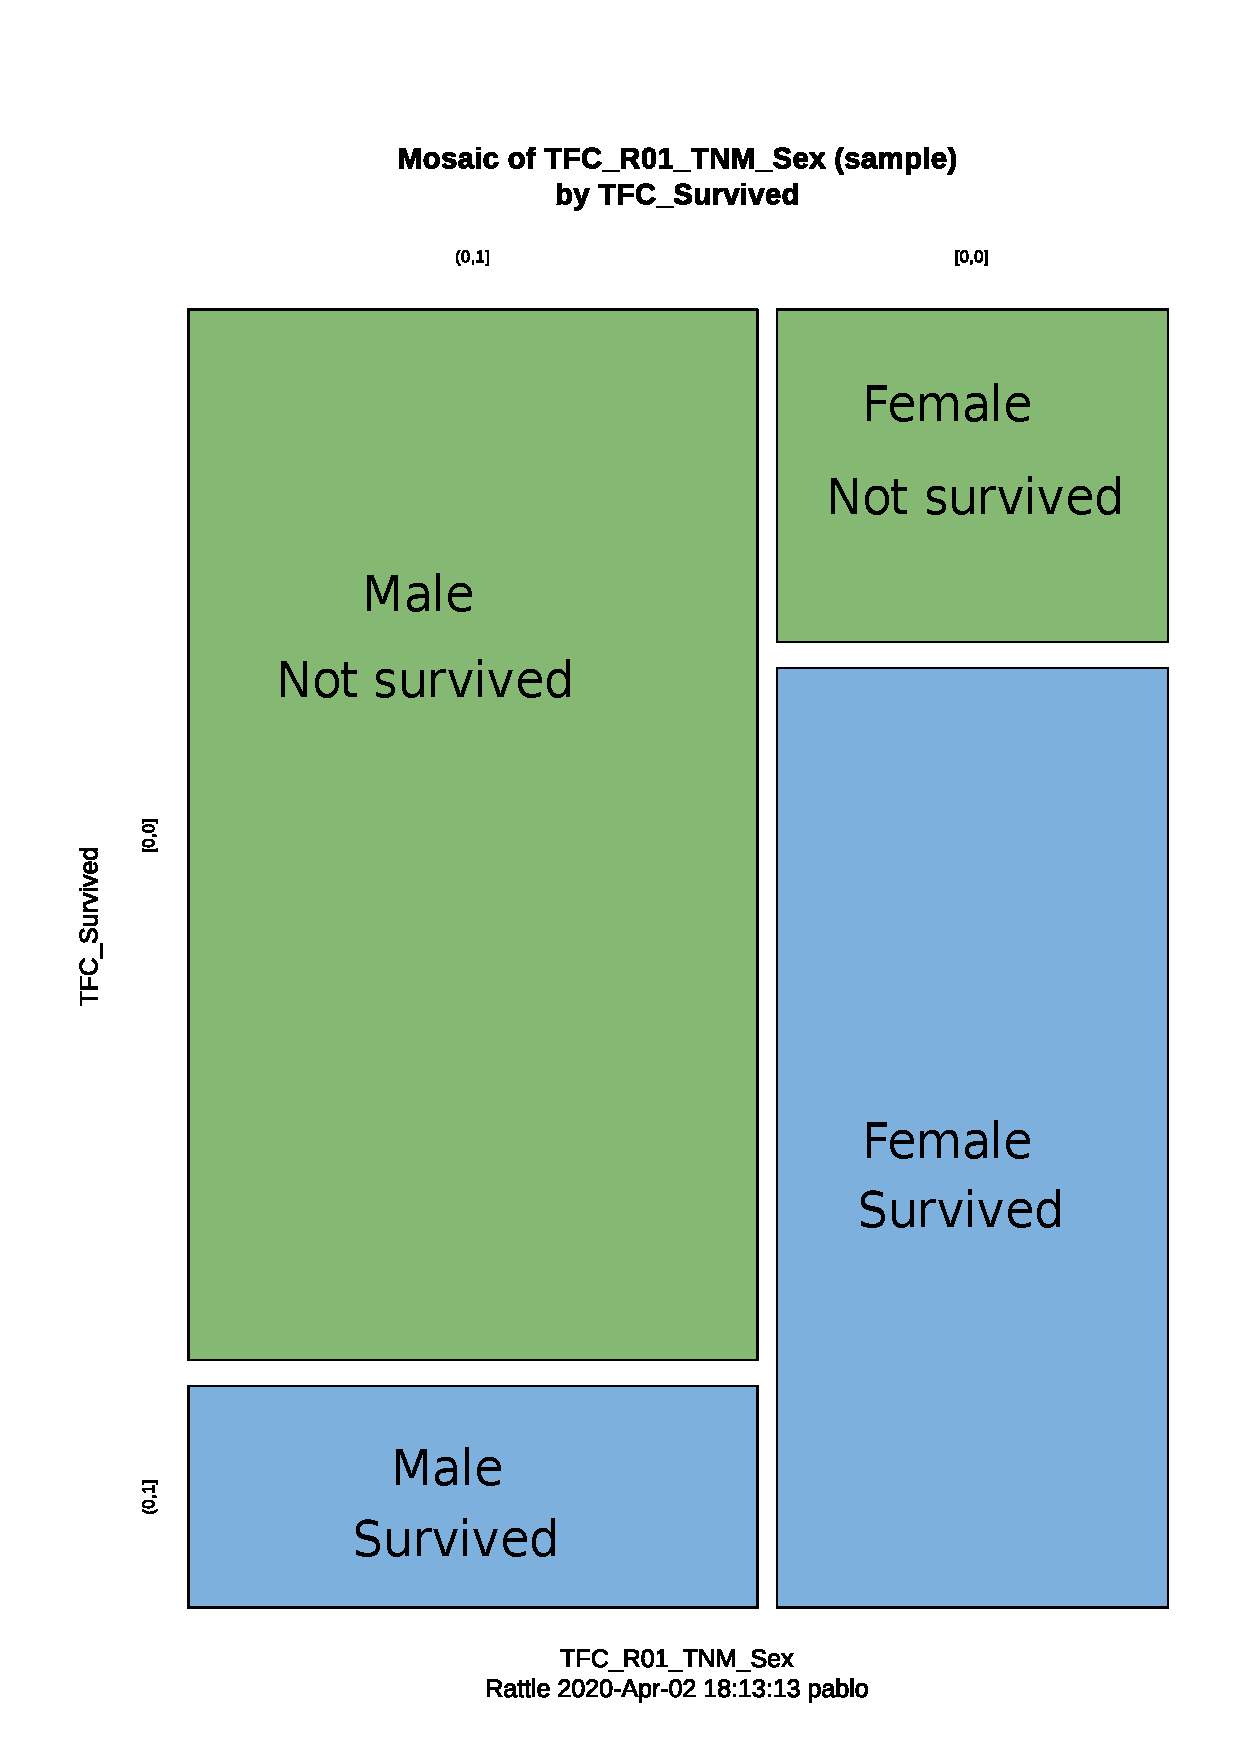
\includegraphics[width=0.5\linewidth]{./img/Rattle-Mosaic-SurvivelByGender}

\hypertarget{references}{%
\section*{References}\label{references}}
\addcontentsline{toc}{section}{References}

\hypertarget{refs}{}
\leavevmode\hypertarget{ref-Wikipedia.titanic.passengers}{}%
Wikipedia contributors. 2020. ``Passengers of the Rms Titanic.'' April
1, 2020.
\url{https://en.wikipedia.org/wiki/Passengers_of_the_RMS_Titanic}.

\leavevmode\hypertarget{ref-WilliamsGraham2011DMwR}{}%
Williams, Graham. 2011. \emph{Data Mining with Rattle and R: The Art of
Excavating Data for Knowledge Discovery}. Use R. New York, NY: Springer
New York.

\end{document}
